\documentclass{article}
\usepackage{graphicx}
\usepackage{float}

\begin{document}
\title{Classification of activities on TPLink router}
\author{Abhinav Narain}
\maketitle
\section{Study of EMI activity on TPLink router}
This study is for EMI activity studied for router~\ref{fig:router} 
\section{Benchmarks}
We want micro benchmarks to suggest how good or bad the technique
we are using. These benchmarks will vary depending on the device if we
want to do activity recognition (for example,camera might run
different applications than a photo-frame.) but might remain the same
for basic activities done by malware.

As suggested by Kyle, I have simulated malware activities, instead of
running actual malware. 

I have done classification for the following activities with the
technique and the results in the section~\ref{sec:technique} and
section~\ref{sec:results}
\begin{itemize}
\item DNS packet flood attack
\item UDP flood attack with payload of 1460 bytes
\item UDP flood attack with payload of 730 bytes
\item Router with default firmware running (Idle)
\item Computation
\end{itemize}

There are set of benchmarks I wanted to do but was unable to proceed
and reasons that it was not possible.
\begin{itemize}
\item Experiments with measurements of L1, L2, L3 caches
  \begin{itemize}
  \item Router does not have many levels of caches as dmesg shows~\ref{subsec:dmesg}
  \end{itemize}
\item copying a file (using Linux command \textit{dd})
  \begin{itemize}
  \item Does not have enough memory to copy files for recording it
  \end{itemize}
\end{itemize}

Figure~\ref{fig:wireless} shows the change in EMI due to turning
hardware switch on or off for the router~\ref{fig:router}. This is
significant change due turning on/off the wireless subsystem which
wasn't present in case of laptop. There is clearly a wide difference
in the proportion of power consumption among the subsystems depending
on the hardware of the device.

\begin{figure}[H]
\centering
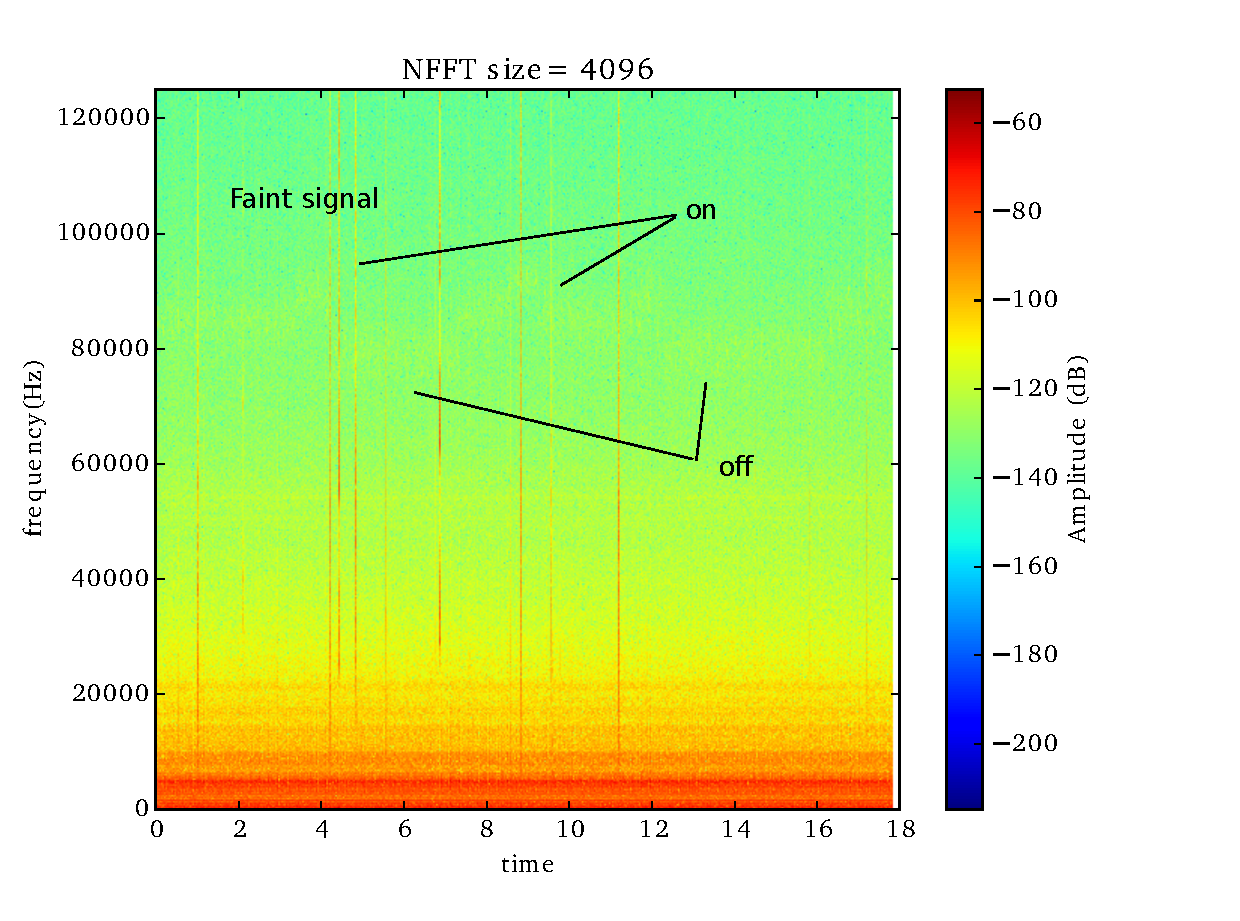
\includegraphics[width=\textwidth]{figures/ww.pdf}
\caption{EMI trace of power-line when the switch powers the wireless
  subsystem on and off. Fs=500kHz}
\label{fig:wireless}
\end{figure}

\section{Technique}\label{sec:technique}
Although there is large spectrum of noise that is produced by the
router, but using the whole spectrum might not be practical (although
techincally correct in the isolated setting) to use in
real setting. The WattsUpDoc(Kevin Fu) work can uses the whole
frequency range as feature set because the setup isolates the device
measurements from the channel measurement with the extra hardware
between the socket and the device.


The EMI trace is segmented period of 10ms as shown in
Fig~\ref{fig:pulse} which is a basic unit of the EMI trace of the
device~\ref{fig:pulse_train} and decomposed using DWT 

\begin{figure}[H]
\centering
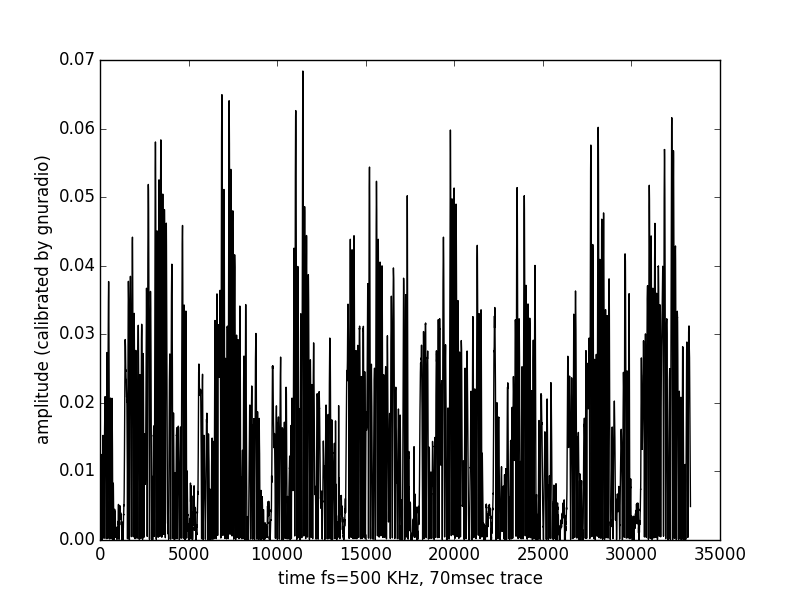
\includegraphics[width=\textwidth]{figures/pulse_train.png}
\caption{Signal trace of router EMI in time domain. This corresponds
  to the alternating bands (cyclo-stationary) in red parts of the spectrogram}
\label{fig:pulse_train}
\end{figure}

\begin{figure}[H]
\centering
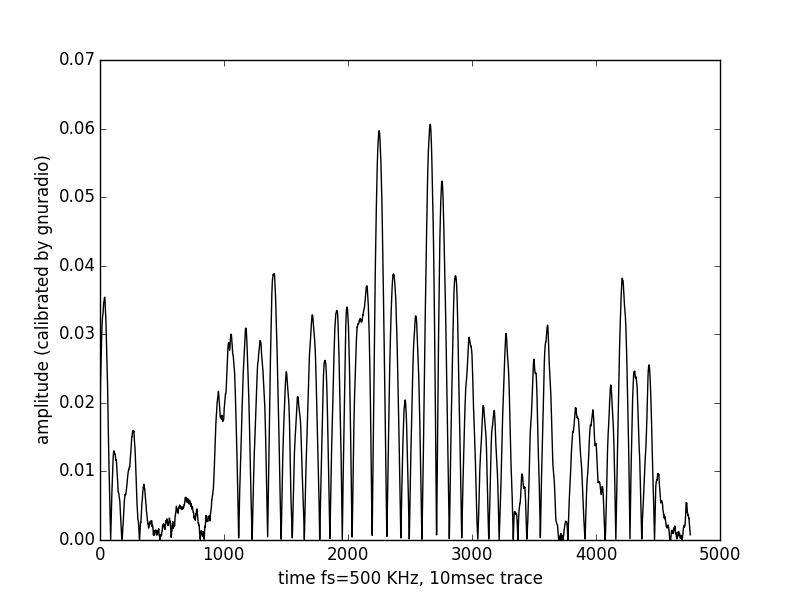
\includegraphics[width=\textwidth]{figures/pulse.png}
\caption{Signal trace of a single segment of router EMI, corresponding
  to one power cycle of the router. This segmented trace is given as a
  feature vector to the classifier}
\label{fig:pulse}
\end{figure}

Each of the the segments  in~\ref{fig:pulse} are used for creating a
feature for the supervised classifier.


To use the coefficients corresponding to the signal referring only to
the specific activity, we have used wavelets as band pass filter to
filter frequency using Discrete Wavelet Transform.

The difference between Discret Wavelet Transform (DWT) and Wavelet
Packet Decomposition (WPT), WPT decomposes the signal space into a
full binary tree, and the basis used are not orthogonal (that is some
nodes will have redundant information). DWT only decomposes the left
half with orthogonal basis tdhe left branch recursively.


While decomposition at every level, each of the algorithms (DWT and
WPT) subsamples while passing through the Low Pass Filter and High Pass
Filter, succesively reducing the number of coefficients by half
and also partitioning the frequency content as shown in figure~\ref{fig:explain}.

Sample rate used in experiments is 500 KHz and the interested frequecies (by visual
inspection of spectrogram) are in 60.25KHz-125 KHz range, and hence we
have selected the DWT coefficients of the second node of the second
row.

\begin{figure}[H]
\centering
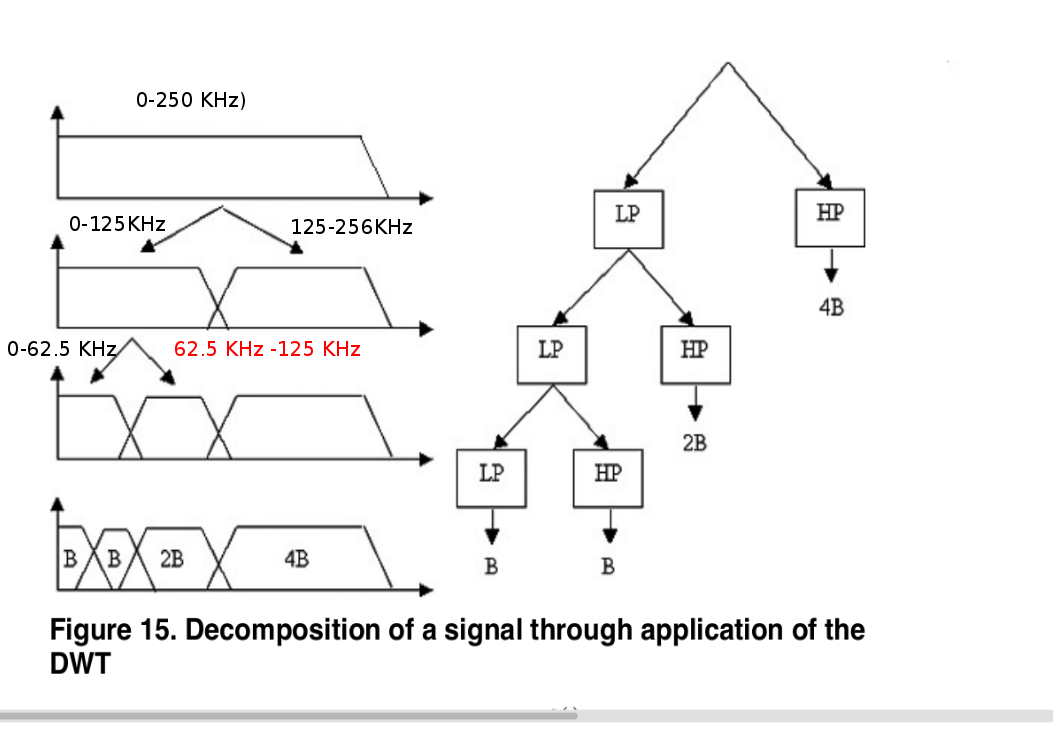
\includegraphics[width=\textwidth]{figures/bp_filter.png}
\caption{Discrete Wavelet Transform. Decomposing the frequency range
  into ranges of values by half at every subsequent level of the
  tree. The sampling frequency is 500KHz and we decompose the maximum
  frequency (250 KHz) at every level.}
\label{fig:explain}
\end{figure}

\section{Results}\label{sec:results}
Spectrograms in Fig~\ref{fig:idle} and Fig~\ref{fig:dns} show the
difference in the change in frequency when DNS flood attack is
performed. The en

Using wider range of frequencies give much better results as indicated
by the precision-recall curve below. Differentiation in packet sizes
might not just be attributed to the change in energy consumption by
the wireless card but also the difference in code generating it.
Although this effect is mitigated in the experiments when the same
code generated UDP packets of different sizes.

\begin{figure}[H]
\centering
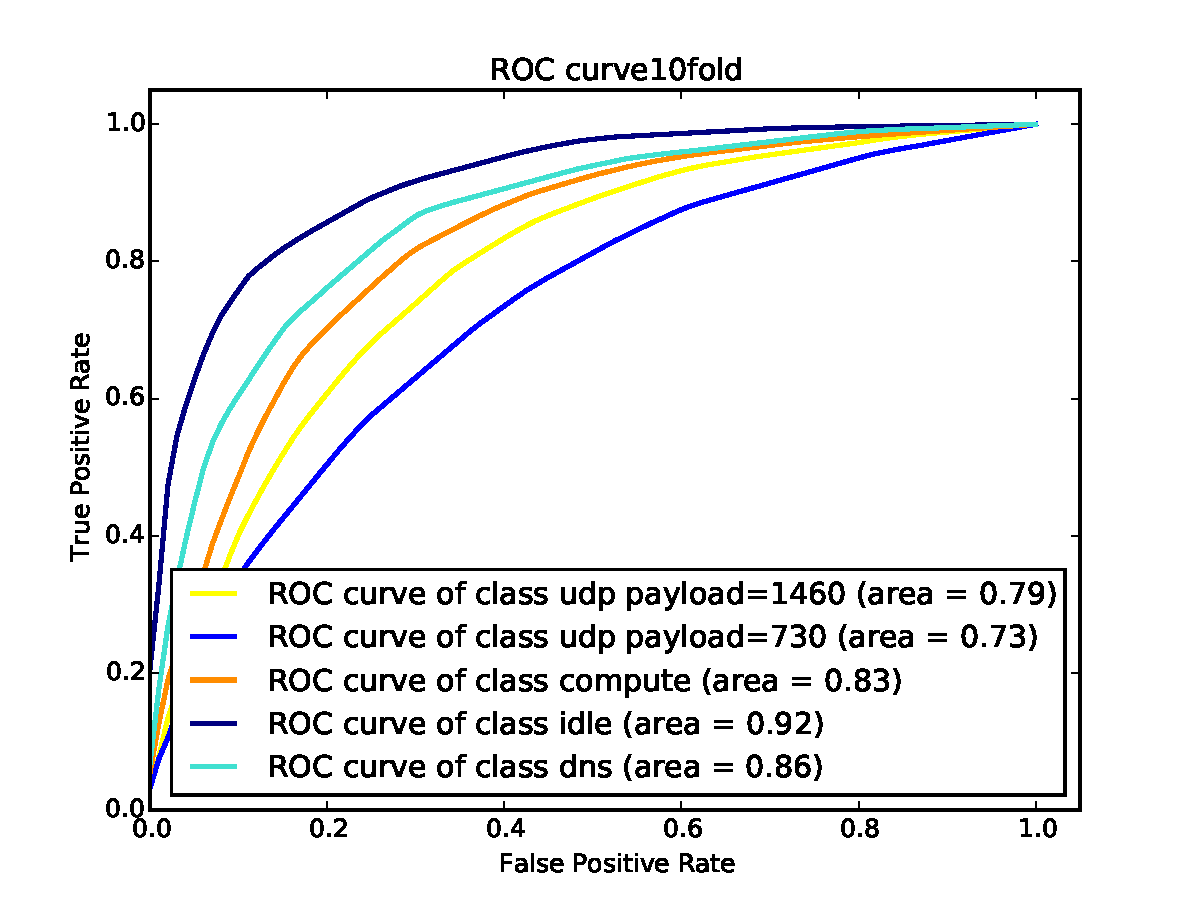
\includegraphics[width=.9\textwidth]{figures/randfor_cAcD_roc_mult_db1.pdf}
\caption{Random Forest Multiclass classifier. This is done using
  Wavelet coefficients at level 2 (on the level marked red in
  Fig~\ref{fig:explain}.}
\label{fig:roc}
\end{figure}

If we take coefficients between between the frequency range of 60-120
KHz as suggested by the spectrogram, we get poor precision-recall
curves, unfortunately there is a lot of information in lower
frequencies which needs to be used for better results.
\begin{figure}[H]
\centering
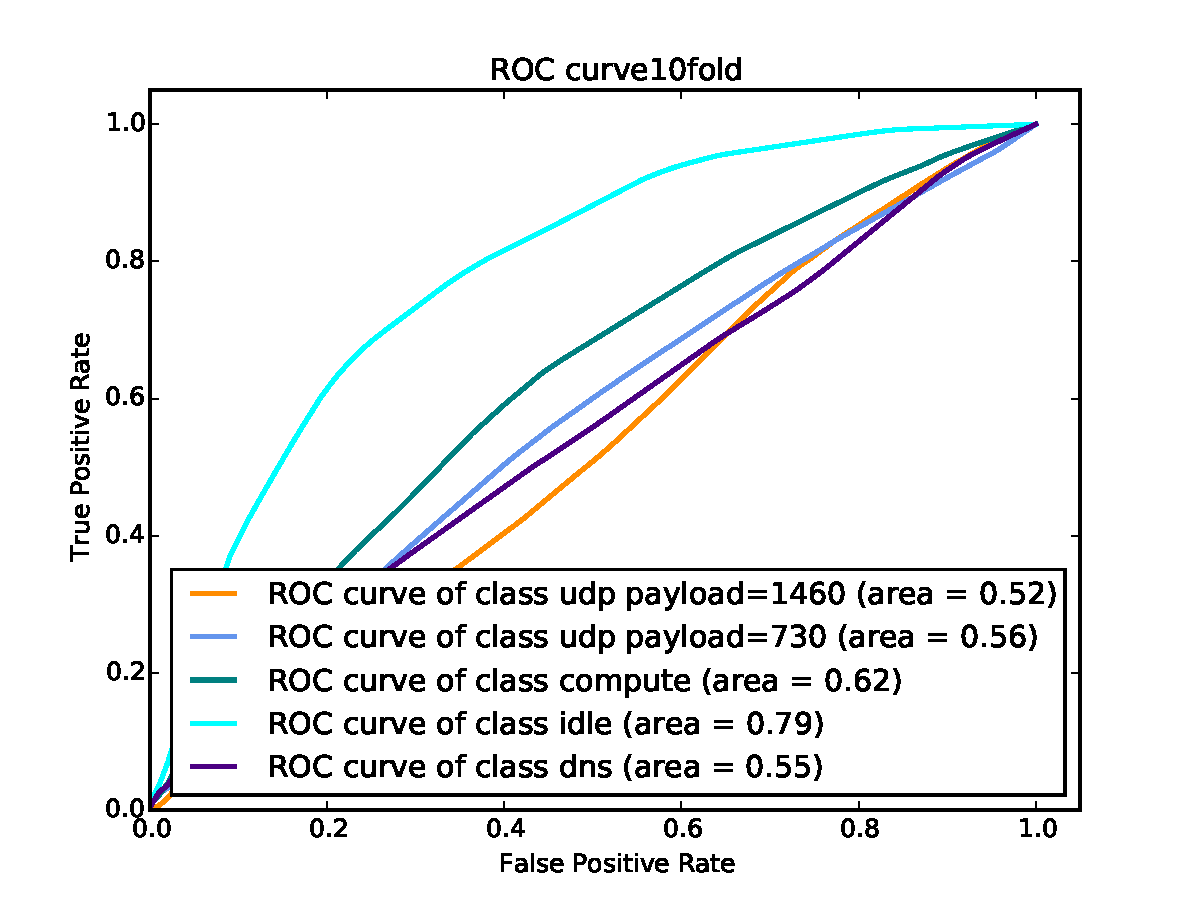
\includegraphics[width=.9\textwidth]{figures/5_rand_forest_roc_mult_bior3_1.pdf}
\caption{Random Forest Multiclass classifier. This is done on the data
  after running a bandpass filter for 60-120KHz to extract the
  frequencies which were visible in spectrogram. The wavelet
  coefficients corresponding to the node marked red in
  Fig~\ref{fig:explain}.}
\label{fig:bandpass_roc}
\end{figure}

\subsection{Comments}
\begin{enumerate}
\item The results are dependent on the hardware. Raspberry Pi did not
  show any activity using our hardware, while the Netgear Router shows
  significant EMI variation for wireless component turned on and the
  packet sizes
\item EMI is not very effective in detecting stealthy malware, which
  has been established in last report on mirai, except when it is
  actively in attack mode.  A  malware can \textit{sleep} for random
  time period (for example in \textit{mirai}) which would evade
  signature detection. I don't think malware would be written to
  especially fool such a detector, but there would be many true
  negatives if the current malware do so already
\item This technique is highly dependent on the hardware
  configuration. Unlike Shwetak's work, where television definitively
  showed correlation between the EMI and movies, we might have to test
  many IoT/computing devices to show on which ones this works
\item I also think, the rate of change of EMI is very slow as the
  television screen and most components are not as fast switching as
  computing devices
\item One might use devices which already use \textit{OpenWrt} to for
  experiments as one can cross-compile and run custom workloads on
  them
\item We can study privacy invasion by measuring EMI when one watches
  a movie. There has been study of packets bitrate coding leaking the
  information about the movie watched on a slingbox (\textit{Usenix Sec 2007:
  Devices That Tell On You: Privacy Trends in Consumer Ubiquitous
  Computing}). This is similar to experiments where Fu et al. have
  used their system to show the web pages visited on a laptop
  (although we do it on a router)
\item We don't know the actual power (in terms of dBm, which is
  something anyone will be interested in knowing), which we don't have
  any calibration device to measure  
\item I had also pursued finding if we could use some bulbs (suggested
  by Kyle in our last meeting) etc. to do a distributed attack from
  bunch of IoT devices together but I was not able to find anything
  useful  
\end{enumerate}

\section{Supplemtary}
\begin{figure}[H]
\centering
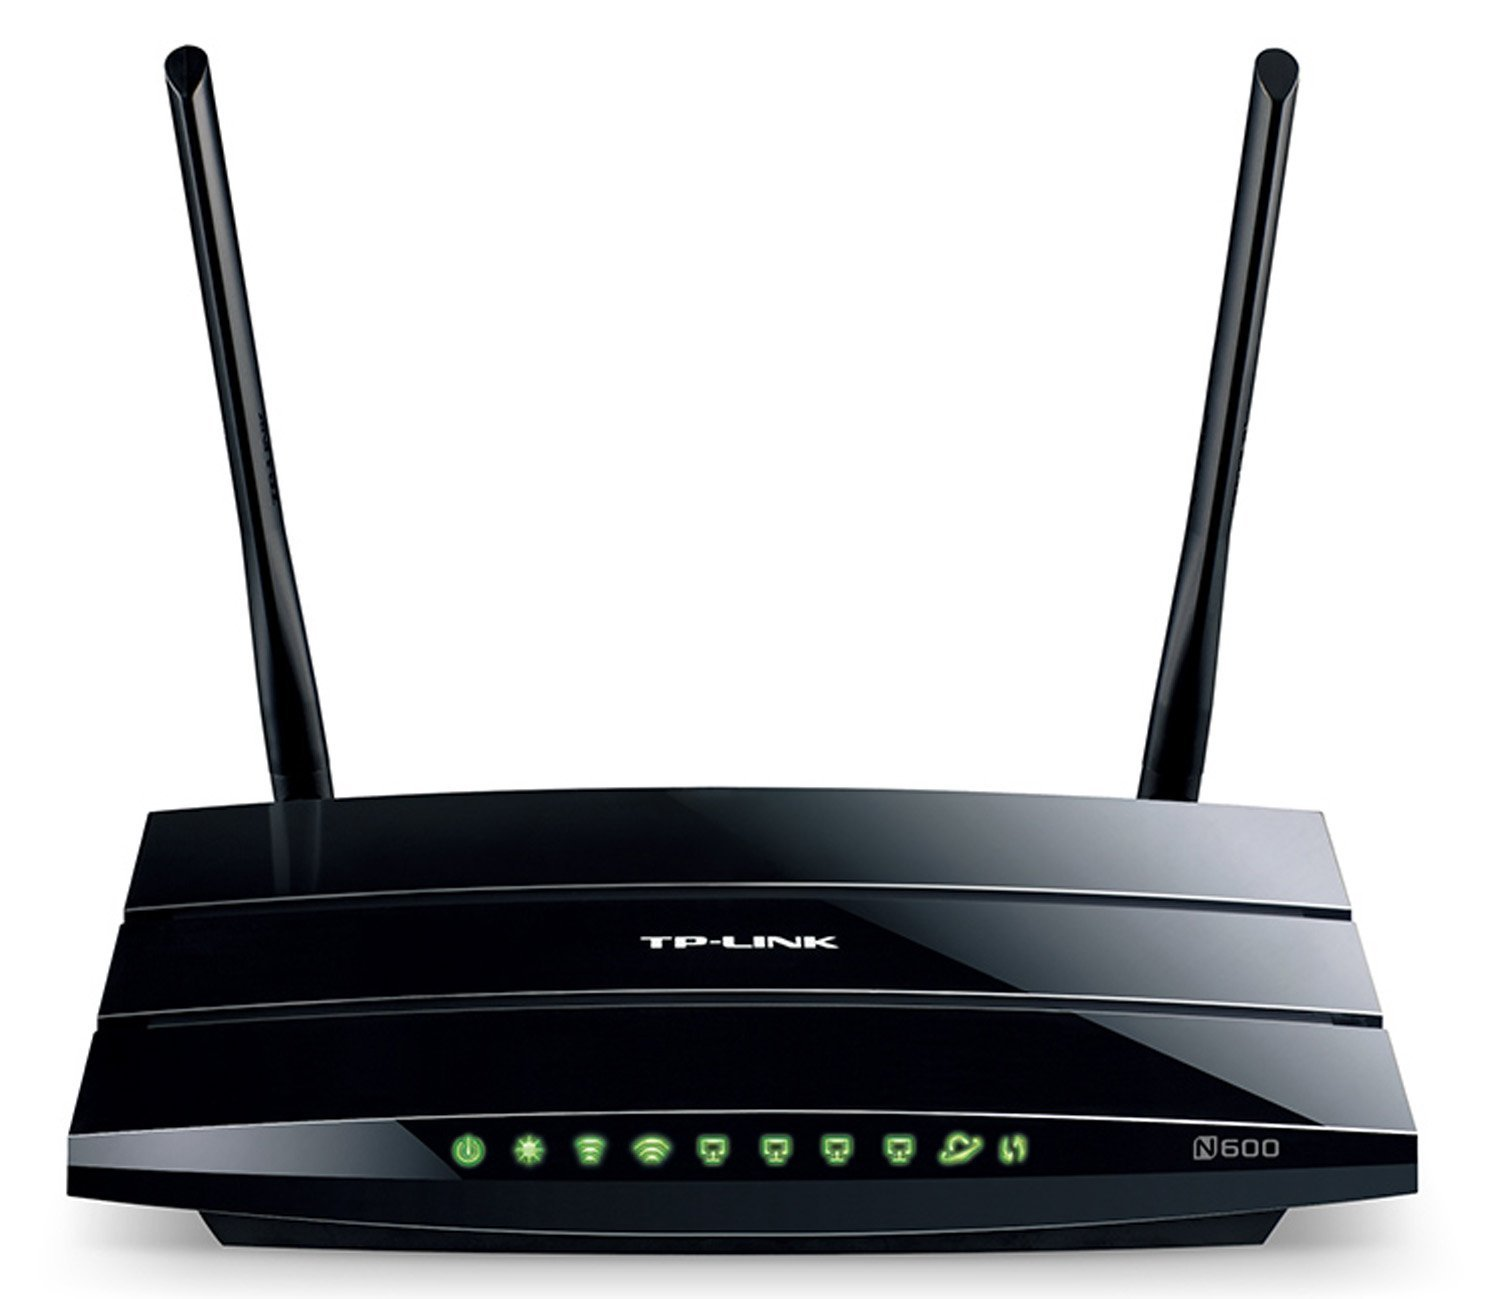
\includegraphics[width=\textwidth]{figures/router.png}
\caption{router used for the study}
\label{fig:router}
\end{figure}


\subsection{Spectrograms of the traces}
\begin{figure}[H]
\centering
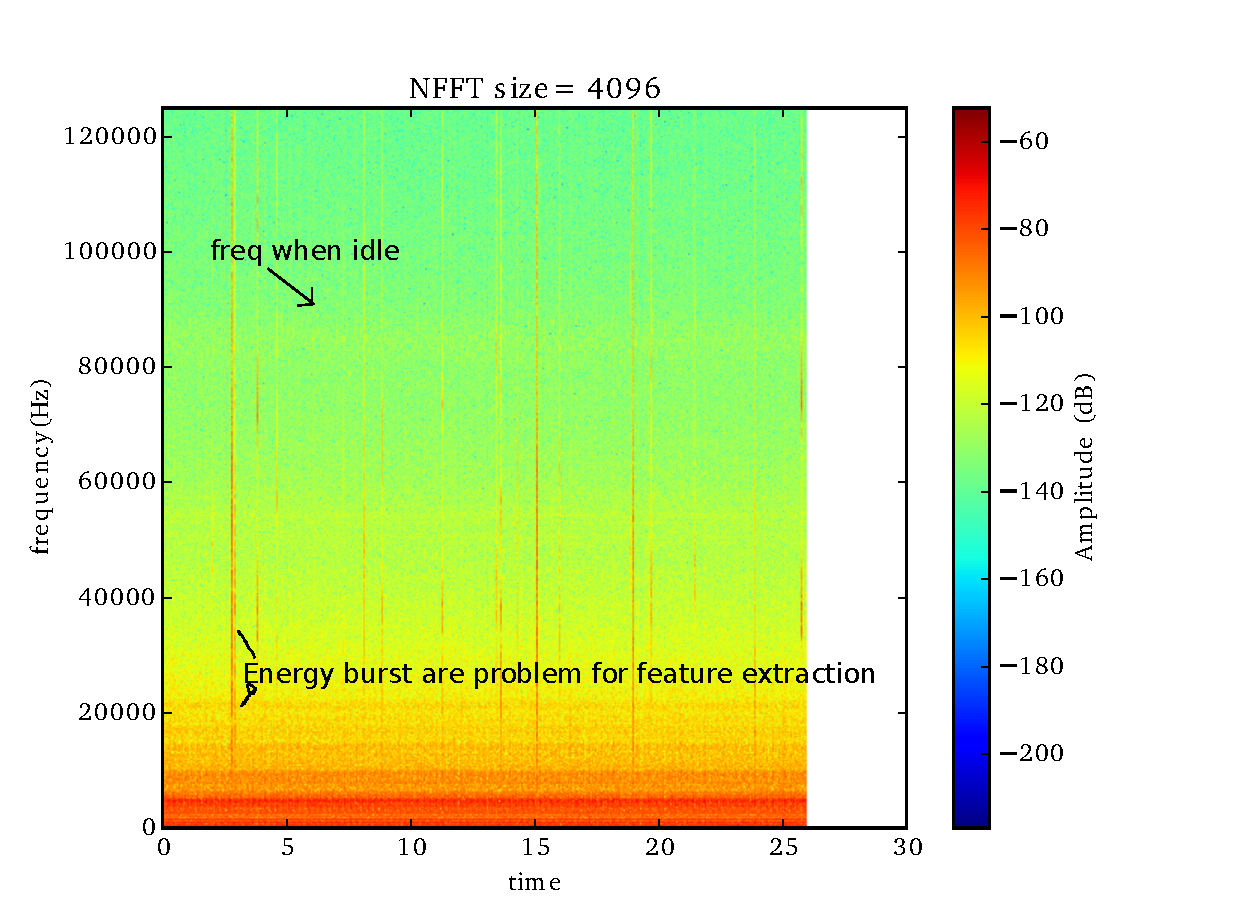
\includegraphics[width=\textwidth]{figures/ii.pdf}
\caption{EMI trace when the router is idle, which means, it is
  not executing any special application/binary installed on it. EMI is
  at ~80KHz. This might be a harmonic for a lower frequency, but it is most
  clear to us and hence indicated in the spectrogram.}
\label{fig:idle}
\end{figure}

\begin{figure}[H]
\centering
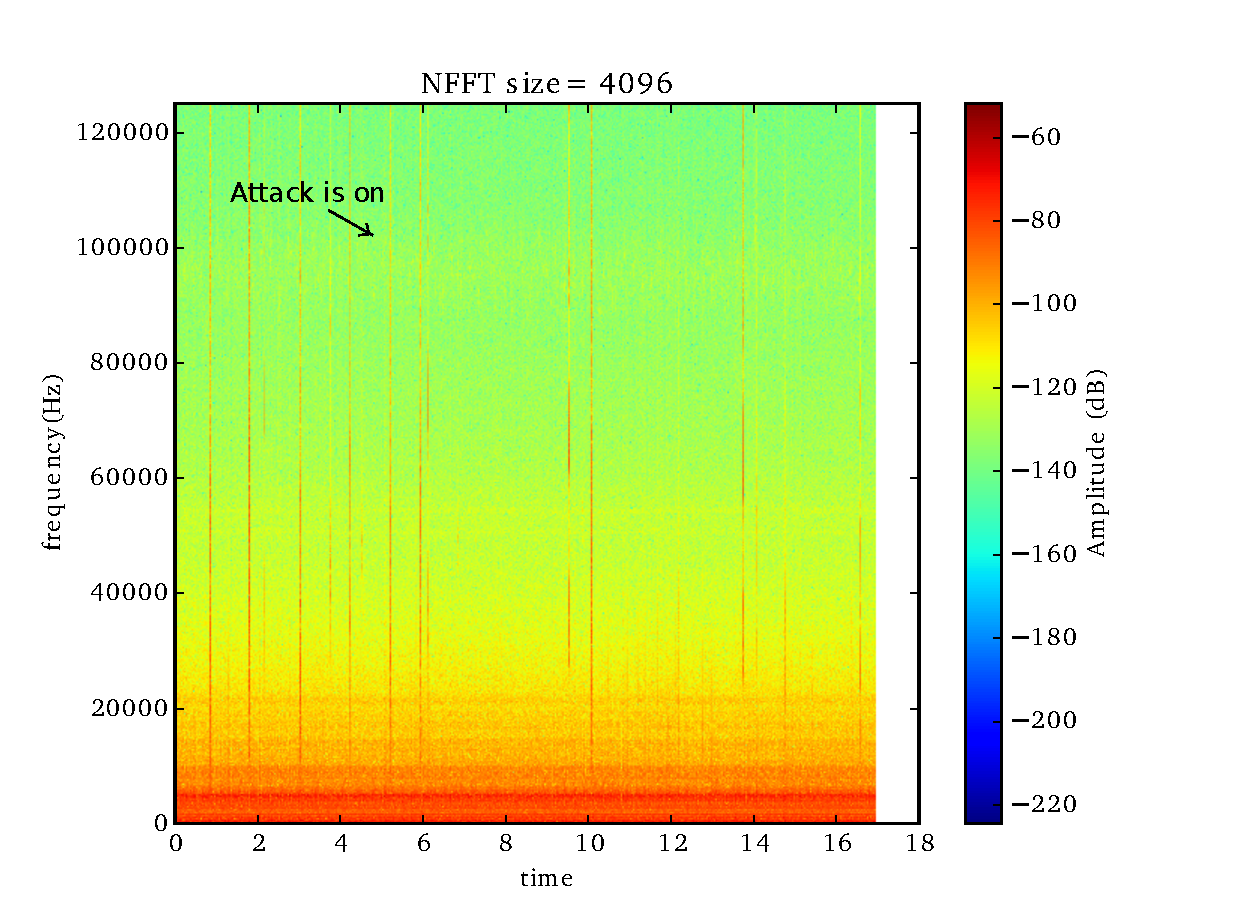
\includegraphics[width=\textwidth]{figures/dd.pdf}
\caption{EMI trace when the router is doing DNS flood attack. The frequency
changes to 100KHz. The same behavior happens when we do UDP flood attack.}
\label{fig:dns}
\end{figure}


\subsection{Time traces of the samples}

\subsection{dmesg output}\label{subsec:dmesg}
\textit{dmesg} output suggesting only L1 cache on
router. \textit{lscpu} command was not found even after going through
whole of menconfig/defconfig files while building \textit{OpenWrt}.

\begin{verbatim}
Cached:             6284 kB 
[    0.000000] Primary instruction cache 64kB, VIPT, 4-way, linesize 32 bytes
[    0.000000] Primary data cache 32kB, 4-way, VIPT, cache aliases, linesize 32 bytes
[    0.000000] Dentry cache hash table entries: 16384 (order: 4, 65536 bytes)
[    0.000000] Inode-cache hash table entries: 8192 (order: 3, 32768 bytes)
[    0.086171] Mount-cache hash table entries: 1024 (order: 0, 4096 bytes)
[    0.093221] Mountpoint-cache hash table entries: 1024 (order: 0, 4096 bytes)
\end{verbatim}

\end{document}
